\documentclass[journal]{IEEEtran}

\usepackage{cite}
\usepackage{amsmath,amssymb,amsfonts}
\usepackage{algorithmic}
\usepackage{graphicx}
\usepackage{textcomp}
\usepackage{xcolor}
\usepackage{booktabs}
\usepackage{multirow}
\usepackage{tabularx}
\usepackage{hyperref}
\usepackage{float}
\usepackage{subcaption}

\begin{document}

\title{TerrainFormer: World Model-Guided Decision Transformer for Autonomous Off-Road Navigation}

\author{Yongzhi~Yang~and~Kenneth~Ricks%
  \thanks{Y.~Yang and K.~Ricks are with the Department of Electrical
    and Computer Engineering, The University of Alabama,
    Tuscaloosa, AL 35487, USA\@.
    E-mail: \texttt{yyang108@crimson.ua.edu}; \texttt{kricks@eng.ua.edu}.}%
  \thanks{Corresponding author: Y.~Yang
    (\texttt{yyang108@crimson.ua.edu}).
    K.~Ricks is a Contributing Author.}%
}

\maketitle

\begin{abstract}
Autonomous navigation in unstructured off-road environments presents fundamental challenges due to terrain heterogeneity, absence of structured road markings, and the necessity for real-time traversability reasoning from raw sensory observations. We present TerrainFormer, a hierarchical framework that integrates a world model for terrain dynamics prediction with a temporal decision transformer for action selection. Our methodology employs a two-phase training paradigm: (1) self-supervised world model pretraining on LiDAR point clouds to learn terrain representations encompassing traversability, elevation, and semantic segmentation; (2) behavioral cloning of the decision transformer conditioned on frozen world model features with temporally-derived goal directions. The world model processes raw 3D LiDAR point clouds through a PointPillars encoder for real-time bird's-eye-view (BEV) projection, followed by a Vision Transformer backbone that produces latent terrain representations. A principal contribution is our cross-dataset generalization paradigm: the world model is trained on separate datasets while the decision transformer is trained on held-out sequences, ensuring zero data overlap between training phases. We introduce automatic goal direction computation from vehicle pose trajectories, enabling the model to learn directionally-conditioned navigation policies. To address class imbalance inherent in off-road driving data, we employ focal loss with inverse-frequency class weighting and action-chunk supervision. Experimental evaluation on the RELLIS-3D dataset achieves 87.31\% test accuracy with 0.7948 macro F1 across all 12 action classes. The world model's predicted future frames produce only a 0.79\% accuracy drop versus ground-truth observations, with 98.82\% action agreement, demonstrating effective cross-dataset generalization for real-time off-road navigation.
\end{abstract}

\begin{IEEEkeywords}
Autonomous navigation, off-road robotics, world models, decision transformers, LiDAR perception, point cloud processing, behavioral cloning, terrain traversability, temporal reasoning, cross-dataset generalization.
\end{IEEEkeywords}

% ============================================================
\section{Introduction}
\label{sec:introduction}
% ============================================================

Autonomous navigation in unstructured off-road environments constitutes a fundamental challenge in mobile robotics and intelligent transportation systems. In contrast to structured urban settings where roads, lane markings, and traffic infrastructure provide strong navigational priors, off-road environments present highly heterogeneous terrain surfaces, dense vegetation, natural obstacles, and environmental conditions that necessitate real-time reasoning about traversability and safe path selection \cite{wellhausen2019, xiao2021}.

Classical approaches to off-road navigation rely on handcrafted terrain classification pipelines and geometric planning algorithms \cite{papadakis2013}. While effective in constrained operational domains, these methods exhibit limited generalization across the diverse conditions encountered in real-world off-road deployment---including mud, gravel, rock formations, dense vegetation, water crossings, and dust. The advent of deep learning has enabled data-driven approaches that learn terrain representations directly from sensor data \cite{maturana2018, wigness2019}; however, most existing methods treat perception and planning as decoupled modules, thereby limiting the capacity to learn end-to-end representations optimized for navigation objectives.

Recent advances in world models \cite{ha2018, hafner2020, hafner2023} and decision transformers \cite{chen2021, zheng2022} present a promising paradigm for learned navigation systems. World models acquire compressed representations of environment dynamics, enabling prediction of future states from current observations and facilitating imagination-based planning. Decision transformers reformulate sequential decision-making as a sequence modeling problem, leveraging the representational capacity of transformer architectures \cite{vaswani2017} for conditioned action prediction. The integration of these paradigms---world models for terrain understanding and decision transformers for action selection---offers a principled framework for autonomous off-road navigation.

In this work, we present \textbf{TerrainFormer}, a hierarchical framework that synthesizes these paradigms for autonomous off-road navigation. Our principal contributions are:

\begin{itemize}
    \item A \textbf{world model architecture} that learns terrain dynamics from raw 3D LiDAR point clouds through self-supervised pretraining, jointly predicting future BEV reconstructions, traversability maps, elevation maps, and semantic segmentation.
    \item A \textbf{decision transformer with action chunking}~\cite{zhao2023act} that builds an 80-token self-attention sequence over world BEV tokens, per-step action history, and learnable chunk queries, predicting $K{=}5$ future actions simultaneously; TemporalEnsemble aggregation of overlapping chunks produces smooth, jitter-free action outputs. Goal directions are derived automatically from vehicle pose trajectories.
    \item A \textbf{real-time PointPillars encoder} that enables end-to-end inference at over 30 FPS, suitable for deployment on robotic platforms with 10 Hz LiDAR sensors.
    \item A \textbf{cross-dataset generalization paradigm} where the world model is trained on LidarDustX \cite{lidardust} and GOOSE-3D \cite{goose2024} while the decision transformer is trained on held-out RELLIS-3D sequences, demonstrating that learned terrain representations transfer across datasets with only 0.79\% accuracy degradation.
    \item A \textbf{focal loss formulation} with automatic inverse-frequency class weighting and label smoothing to address severe class imbalance in off-road action distributions, improving minority class detection.
    \item A \textbf{predictive evaluation protocol} that quantifies the impact of world model prediction quality on downstream action selection, achieving 98.82\% prediction agreement between current and predicted frame conditions.
\end{itemize}

% ============================================================
\section{Related Work}
\label{sec:related_work}
% ============================================================

\subsection{Off-Road Terrain Perception}

LiDAR-based terrain perception has been studied extensively for autonomous off-road navigation. Early methods relied on geometric features such as slope, roughness, and step height for terrain classification \cite{papadakis2013}. More recent approaches employ deep learning on point clouds \cite{qi2017, qi2017b} or bird's-eye-view (BEV) projections \cite{zhou2018, lang2019} to learn terrain representations. The RELLIS-3D dataset \cite{jiang2021} provides annotated LiDAR scans across diverse off-road terrain types, enabling supervised learning of terrain semantics.

Traversability estimation is a key component of off-road navigation. Methods range from geometry-based approaches \cite{sock2016} to learning-based frameworks that predict traversability from point clouds or images \cite{wellhausen2019, frey2023}. Self-supervised approaches have shown particular promise, learning traversability from proprioceptive signals during traversal \cite{castro2023, frey2024}.

\subsection{World Models for Robotics}

World models learn compact representations of environment dynamics, enabling an agent to predict future states and plan accordingly. Dreamer \cite{hafner2020} and DreamerV3 \cite{hafner2023} demonstrated the effectiveness of world models for continuous control tasks, learning latent dynamics models that support imagination-based planning. MILE \cite{hu2022} applied world models to urban autonomous driving, jointly predicting future BEV semantic maps and planning trajectories.

In the context of 3D environments, Point Cloud World Models \cite{yang2023} and related approaches have explored predicting future 3D scenes from LiDAR observations. Our work extends this direction to off-road environments, where terrain dynamics are more complex and varied than structured road scenes.

\subsection{Decision Transformers}

The Decision Transformer \cite{chen2021} reformulated offline reinforcement learning as a sequence modeling problem, conditioning action generation on desired returns. Subsequent work has extended this framework with trajectory transformers \cite{janner2021}, online fine-tuning \cite{zheng2022}, and multi-modal conditioning \cite{xu2022}. In the driving domain, transformers have been applied to trajectory prediction \cite{nayakanti2023} and end-to-end planning \cite{hu2023}.

Our approach differs from prior decision transformer work in three key aspects: (1) we condition decisions on learned world model representations rather than raw observations, enabling abstraction of terrain features; (2) we adopt action chunking~\cite{zhao2023act} with TemporalEnsemble over a full-sequence token architecture that attends jointly to spatial (BEV world tokens), temporal (action-history tokens), and predictive (chunk query) tokens; and (3) we use discrete navigation actions with automatically-derived goal directions suited to off-road settings rather than continuous trajectory waypoints typical of urban driving.

\subsection{Behavioral Cloning for Navigation}

Behavioral cloning (BC) learns policies directly from expert demonstrations \cite{pomerleau1989, bojarski2016}. While BC suffers from distribution shift in theory, it remains a practical and effective approach when paired with data augmentation and appropriate action representations \cite{codevilla2018}. For off-road navigation, BC has been applied using various input modalities including RGB images \cite{kahn2021}, LiDAR \cite{wigness2019}, and multi-modal inputs \cite{triest2023}. Our work employs BC for the decision transformer training phase, using expert trajectories from the RELLIS-3D dataset.

% ============================================================
\section{Methodology}
\label{sec:methodology}
% ============================================================

TerrainFormer comprises four principal components arranged in a hierarchical pipeline (Fig.~\ref{fig:architecture}): (1) a LiDAR encoder that processes raw 3D point clouds into dense features, (2) a BEV projection module that creates spatial feature maps suitable for downstream processing, (3) a world model that learns terrain dynamics and latent representations through self-supervised pretraining, and (4) a temporal decision transformer that predicts discrete navigation actions conditioned on temporal context and automatically-derived goal directions. Training proceeds in two phases: self-supervised world model pretraining (Phase~1) using multi-dataset LiDAR observations, followed by behavioral cloning for the temporal decision transformer (Phase~2) on held-out sequences.

\begin{figure*}[t]
    \centering
    
\includegraphics[width=\linewidth]{terrainformer_flowchart.png}
    \caption{%
        TerrainFormer system flow chart.
        \textbf{Data pipeline} (blue): Phase~1 uses LidarDustX and GOOSE-3D for self-supervised world model pretraining (no RELLIS-3D); Phase~2 loads RELLIS-3D sequences with action chunk labels ($K{=}5$) for behavioral cloning.
        \textbf{Shared encoder + world model} (green/peach): PointPillars projects raw point clouds to a $64{\times}256{\times}256$ BEV feature map; the ViT-based world model compresses it to a global feature $(B,512)$ and 64 latent tokens $(B,64,512)$.
        \textbf{Phase 1} (yellow): four self-supervised prediction heads (traversability, elevation, semantics, future frames) are trained jointly; the encoder and world model are \emph{frozen} in Phase 2.
        \textbf{Phase 2} (lavender): the DecisionTransformer builds an 80-token sequence $[\text{context}(1)\,|\,\text{world}(64)\,|\,\text{history}(10)\,|\,\text{chunk queries}(5)]$, applies 4 layers of self-attention, and decodes the context token into current-step action logits and the last five tokens into $K{=}5$ chunk logits simultaneously.
        \textbf{Inference} (teal): TemporalEnsemble averages overlapping chunk predictions across $K$ consecutive frames with exponential decay weighting~($\lambda{=}0.9$) to produce smooth, jitter-free action outputs from the 12-class forward-only action vocabulary.
        \textbf{Notation} --- $B$: batch size (number of samples processed simultaneously);
        $N$: number of LiDAR points per scan (up to 65,536);
        $C$: number of BEV feature channels (64);
        $H{\times}W$: BEV spatial resolution ($256{\times}256$ pixels, covering $100\,\text{m}{\times}100\,\text{m}$);
        $d$: world model embedding dimension (512);
        $K$: action chunk size --- number of future actions predicted per frame ($K{=}5$);
        $T$: action history length (10 past steps);
        $L$: total transformer sequence length ($L{=}80$ tokens);
        $\lambda$: TemporalEnsemble exponential decay weight ($\lambda{=}0.9$, higher weight for more recent predictions);
        $A$: number of discrete action classes ($A{=}12$).
        Tensor shapes are written as $(B,\,\text{tokens},\,d)$ or $(B,\,d)$ for vectors.
    }
    \label{fig:architecture}
\end{figure*}

\subsection{LiDAR Encoder}
\label{sec:lidar_encoder}

The LiDAR encoder processes raw 3D point clouds of up to $N = 65{,}536$ points, where each point has four features $(x, y, z, i)$ representing spatial coordinates and intensity. We employ a PointPillars-based encoder \cite{lang2019} that directly converts point clouds to BEV features, chosen for its architectural alignment with our BEV-centric pipeline and real-time performance characteristics.

\subsubsection{PointPillars Architecture}
The encoder operates as follows:

\begin{enumerate}
    \item \textbf{Pillarization}: Points are discretized into vertical pillars on a $256 \times 256$ BEV grid covering $100\,\text{m} \times 100\,\text{m}$ ($x, y \in [-50, 50]$\,m). Each pillar aggregates up to 32 points.
    \item \textbf{Feature Augmentation}: Each point is augmented with 5 additional features: $(x_c, y_c, z_c)$ offset from pillar centroid and $(x_p, y_p)$ offset from pillar geometric center, yielding 9-dimensional input.
    \item \textbf{Pillar Feature Network}: A two-layer MLP ($9 \rightarrow 64 \rightarrow 64$) encodes per-point features, followed by max-pooling within each pillar using vectorized \texttt{scatter\_reduce} operations.
    \item \textbf{BEV Backbone}: Two $3 \times 3$ convolutional layers with BatchNorm and ReLU refine the spatial features.
\end{enumerate}

The PointPillars encoder achieves ${\sim}5$\,ms latency on modern GPUs, enabling real-time inference at 10 Hz LiDAR rates with ample margin for downstream processing.

\subsubsection{Encoder Design Rationale}
We considered alternative architectures including PointNet++ \cite{qi2017b}, which offers hierarchical set abstraction for fine-grained local geometry learning. However, PointPillars was selected for three reasons: (1) \textbf{architectural alignment}---PointPillars produces BEV features directly, matching the world model's expected input without intermediate projection layers; (2) \textbf{latency}---PointPillars achieves $5\times$ lower encoder latency, critical for real-time navigation at 10\,Hz; (3) \textbf{compensating capacity}---the 6-layer Dynamics Transformer provides sufficient representational capacity to learn fine-grained terrain patterns that hierarchical point encoders would capture at the encoder level.

Table~\ref{tab:encoder_comparison} compares the two encoder architectures, including per-component FPS. PointPillars achieves ${\sim}200$\,FPS at the encoder stage (vs.\ ${\sim}40$\,FPS for PointNet++), and the full TerrainFormer pipeline runs at ${\sim}50$\,FPS end-to-end. A hypothetical PointNet++ variant would achieve only ${\sim}25$\,FPS end-to-end, falling below the 30\,FPS threshold required for responsive real-time navigation and exceeding the 100\,ms frame budget when combined with downstream processing.

\begin{table}[h]
\caption{LiDAR Encoder Comparison: PointPillars (Ours) vs.\ PointNet++}
\label{tab:encoder_comparison}
\centering
\begin{tabular}{lcc}
\toprule
Metric & PointPillars (Ours) & PointNet++ \\
\midrule
Encoder latency   & ${\sim}5$\,ms          & ${\sim}25$\,ms \\
Encoder FPS       & ${\sim}200$\,FPS       & ${\sim}40$\,FPS \\
Full-system FPS   & ${\sim}50$\,FPS        & ${\sim}25$\,FPS \\
Parameters        & 0.15\,M                & 1.48\,M \\
Output format     & BEV (direct)           & Point features \\
BEV projection    & Built-in               & Requires additional \\
TensorRT support  & Full                   & Limited \\
Real-time (10\,Hz) & \checkmark            & $\times$ \\
\bottomrule
\end{tabular}
\smallskip
\parbox{\columnwidth}{\footnotesize Full-system FPS computed as $1000\,\text{ms}\,/\,(t_\text{enc}+10+5)$, where $10$\,ms and $5$\,ms are the world model and decision transformer latencies respectively.}
\end{table}

The $5\times$ latency advantage of PointPillars (${\sim}5$\,ms vs.\ ${\sim}25$\,ms) is critical for real-time off-road navigation, where rapid terrain changes and dynamic obstacles require low-latency perception-to-action pipelines. PointNet++'s hierarchical set abstraction, while theoretically richer for local geometry, adds computational overhead that precludes real-time operation when combined with world model inference (${\sim}10$\,ms) and decision transformer processing (${\sim}5$\,ms). Empirically, for BEV-based downstream tasks, PointPillars consistently matches PointNet++ performance on established benchmarks while enabling TensorRT optimization for embedded deployment.

\subsubsection{BEV Output}
The encoder produces a BEV feature map $\mathbf{F}_\text{BEV} \in \mathbb{R}^{64 \times 256 \times 256}$ and a global feature vector $\mathbf{z}_\text{encoder} \in \mathbb{R}^{1024}$ via adaptive pooling followed by linear projection.

\subsection{World Model}
\label{sec:world_model}

The world model learns to predict terrain dynamics and extract rich representations from BEV features through self-supervised pretraining. It consists of three components: a terrain tokenizer, a dynamics transformer, and a latent state module.

\subsubsection{Terrain Tokenizer}
The BEV feature map $\mathbf{F}_\text{BEV}$ is divided into non-overlapping patches of size $16 \times 16$ pixels, yielding $P = (256/16)^2 = 256$ patches. Each patch is projected to a token of dimension $d = 512$ via a convolutional embedding layer. Learned positional encodings $\mathbf{E}_\text{pos} \in \mathbb{R}^{256 \times 512}$ and a learnable \texttt{[CLS]} token are prepended, producing an input sequence of $257$ tokens.

\subsubsection{Dynamics Transformer}
The token sequence is processed by a 6-layer transformer encoder with the following configuration per layer: $d_\text{model} = 512$, $h = 8$ attention heads, head dimension $d_k = 64$, MLP ratio $4\times$ (intermediate dimension $2048$), and dropout rate $0.1$. The architecture uses pre-norm (LayerNorm before attention and MLP) following the convention of Vision Transformers \cite{dosovitskiy2021}.

\subsubsection{Latent State Compression}
To produce a compact representation for the decision transformer, we employ a cross-attention-based compression module. A set of $64$ learnable latent queries $\mathbf{Q}_\text{latent} \in \mathbb{R}^{64 \times 512}$ attend to the $257$ transformer output tokens via multi-head cross-attention ($h = 8$ heads), producing compressed latent tokens $\mathbf{Z} \in \mathbb{R}^{64 \times 512}$. A global feature vector $\mathbf{z}_\text{global} \in \mathbb{R}^{512}$ is obtained via mean pooling over the latent tokens followed by a linear projection.

\subsubsection{Prediction Heads}
Four parallel prediction heads decode the latent representations for self-supervised training:

\begin{enumerate}
    \item \textbf{Future Reconstruction}: Predicts the next 5 frames' BEV features at patch resolution, output $\mathbb{R}^{5 \times 64 \times 16 \times 16}$.
    \item \textbf{Traversability}: Transposed convolution upsampling ($4\times$) to produce a binary traversability map $\mathbb{R}^{1 \times 256 \times 256}$ with sigmoid activation.
    \item \textbf{Elevation}: Same architecture, predicting continuous elevation values $\mathbb{R}^{1 \times 256 \times 256}$.
    \item \textbf{Semantics}: Transposed convolution upsampling to produce per-class logits $\mathbb{R}^{C \times 256 \times 256}$ where $C = 20$ for RELLIS-3D semantic classes.
\end{enumerate}

\subsection{Decision Transformer}
\label{sec:decision_transformer}

The decision transformer predicts discrete navigation actions using a token-sequence architecture that provides full cross-attention between spatial world features, temporal action history, and learnable future-action query tokens.

\subsubsection{Token Sequence Architecture}
Inspired by action chunking~\cite{zhao2023act}, the model simultaneously predicts the next $K{=}5$ actions per frame rather than a single step, improving temporal coherence and enabling anticipatory look-ahead. The transformer processes a fixed-length sequence of $L{=}80$ tokens:
\begin{equation}
    \mathbf{X} = \bigl[\mathbf{c};\;\mathbf{W}_{1:64};\;\mathbf{A}_{1:10};\;\mathbf{Q}_{1:5}\bigr]
    \;\in \mathbb{R}^{80 \times 384}
\end{equation}
where $\mathbf{c} \in \mathbb{R}^{384}$ is a fused \emph{context token}, $\mathbf{W}_{1:64}$ are projected world latent tokens (BEV spatial features), $\mathbf{A}_{1:10}$ are per-step action history embeddings (temporal features), and $\mathbf{Q}_{1:5}$ are $K$ learnable \emph{chunk query} tokens that represent the $K$ future action predictions.

Learnable positional embeddings $\mathbf{E}_\text{pos} \in \mathbb{R}^{80 \times 384}$ are added to the full sequence to encode token order.

\subsubsection{Context Aggregator}
The context token $\mathbf{c}$ fuses four information sources through a two-layer MLP followed by cross-attention over the world latent tokens $\mathbf{Z}$:
\begin{itemize}
    \item \textbf{World global feature}: $\mathbf{z}_\text{global} \in \mathbb{R}^{512}$, linearly projected to $\mathbb{R}^{384}$.
    \item \textbf{Vehicle state}: $\mathbf{s} \in \mathbb{R}^{6}$ encoding velocity $(v_x, v_y)$, angular velocity $\omega$, and orientation (pitch, roll, yaw).
    \item \textbf{Goal direction}: $\mathbf{g} \in \mathbb{R}^{2}$ (Section~\ref{sec:goal_direction}).
    \item \textbf{Action aggregate}: $\mathbf{e}_a \in \mathbb{R}^{128}$, mean-pooled over 10 per-step action embeddings.
\end{itemize}
\begin{equation}
    \mathbf{c} = \text{CrossAttn}\!\left(\text{MLP}_\text{fuse}([\text{proj}(\mathbf{z}_\text{global}); \mathbf{e}_s; \mathbf{e}_g; \mathbf{e}_a]),\;\mathbf{Z}\right) \in \mathbb{R}^{384}
\end{equation}

\subsubsection{Token Projections}
World latent tokens $\mathbf{Z} \in \mathbb{R}^{64 \times 512}$ are projected to $\mathbb{R}^{64 \times 384}$ via a linear layer. Action history embeddings are produced per-step (preserving temporal structure) and projected to $\mathbb{R}^{10 \times 384}$ via a separate linear layer. Chunk queries $\mathbf{Q} \in \mathbb{R}^{5 \times 384}$ are learnable parameters initialized with truncated-normal distribution ($\sigma{=}0.02$).

\subsubsection{Transformer Backbone}
The 80-token sequence is processed by a 4-layer transformer with $d_\text{model}{=}384$, $h{=}6$ attention heads, head dimension $d_k{=}64$, MLP ratio $4\times$, and dropout $0.1$, using pre-norm (LayerNorm before attention and MLP). Full self-attention over all 80 tokens enables each chunk query to attend simultaneously to BEV spatial context (world tokens) and temporal action history (action tokens), providing richer conditioning than single-token architectures.

\subsubsection{Output Heads}
\begin{enumerate}
    \item \textbf{Current-step action}: The context token output $\mathbf{x}_0 \in \mathbb{R}^{384}$ is decoded by an action head (MLP $384{\to}12$), a confidence head (MLP $384{\to}1$ with sigmoid), and an auxiliary traversability head (MLP $384{\to}1$ with sigmoid).
    \item \textbf{Action chunk}: Each of the last $K{=}5$ output tokens $\mathbf{x}_{-5:} \in \mathbb{R}^{5 \times 384}$ is independently decoded by the shared action head, yielding chunk logits $\in \mathbb{R}^{K \times 12}$.
\end{enumerate}

\subsubsection{Temporal Ensembling at Inference}
At inference, each frame produces a $K{=}5$ action chunk. Overlapping chunks from the last $K$ consecutive frames are aggregated via \emph{TemporalEnsemble}~\cite{zhao2023act} using exponential-decay weighting:
\begin{equation}
    \hat{a}_t = \arg\max_a \;\frac{\displaystyle\sum_{k=0}^{K-1} \lambda^k \cdot \text{chunk}_{t-k}[k]}
                                  {\displaystyle\sum_{k=0}^{K-1} \lambda^k},
    \quad \lambda = 0.9
\end{equation}
where $\text{chunk}_{t-k}[k]$ is the $k$-th step prediction from the chunk generated $k$ frames ago. More recent predictions receive higher weight. This averaging suppresses prediction jitter and smooths action transitions without latency overhead.

\subsection{Action Space}
\label{sec:action_space}

We define a discrete action space of 12 forward-motion actions that combines speed and steering commands, derived from continuous vehicle poses via velocity and turn-rate thresholding (Table~\ref{tab:action_space}). The action space is designed specifically for forward-only driving scenarios characteristic of the RELLIS-3D dataset, which contains no backward motion. Actions are classified using a turn-first approach: turn rate magnitude determines the action category, with forward-speed actions reserved for minimal-turn scenarios.

\begin{table}[h]
\caption{Discrete Action Space (12 Forward-Motion Actions)}
\label{tab:action_space}
\centering
\begin{tabular}{clcl}
\toprule
ID & Action & ID & Action \\
\midrule
0 & Stop & 6 & Left slight \\
1 & Forward slow & 7 & Right slight \\
2 & Forward medium & 8 & Right medium \\
3 & Forward fast & 9 & Right sharp \\
4 & Left sharp & 10 & Forward left \\
5 & Left medium & 11 & Forward right \\
\bottomrule
\end{tabular}
\end{table}

Action labels are derived from ground-truth pose sequences by computing linear velocity and turn rate between consecutive frames ($\Delta t = 0.1$\,s). Using a turn-first classification approach, turn rate magnitude is evaluated first: sharp ($|\omega| \geq 0.6$ rad/s), medium ($0.3$--$0.6$), slight ($0.1$--$0.3$), or minimal ($< 0.1$). Turn actions (4--9) are assigned regardless of velocity; forward-speed actions (0--3) apply only when $|\omega| < 0.1$. Combined actions (10--11) represent fast forward motion ($v \geq 1.0$ m/s) with sharp turning. Since RELLIS-3D contains exclusively forward driving trajectories (no backward motion), the action space excludes backward-related actions, simplifying the classification task while maintaining expressiveness for off-road navigation.

\subsection{Goal Direction Computation}
\label{sec:goal_direction}

A critical component of directionally-conditioned navigation is the goal direction input, which informs the model where the vehicle should navigate. Rather than relying on externally-provided waypoints, we compute goal directions automatically from the vehicle's future trajectory encoded in the pose sequence.

For each frame $t$, the goal direction $\mathbf{g}_t \in \mathbb{R}^2$ is computed as the normalized displacement vector from the current position to a future position (lookahead $k=5$ frames), expressed in the vehicle's local coordinate frame:

\begin{equation}
    \mathbf{d}_t = \mathbf{p}_{t+k} - \mathbf{p}_t
\end{equation}
\begin{equation}
    \mathbf{g}_t = \mathbf{R}(-\psi_t) \cdot \frac{\mathbf{d}_t}{\|\mathbf{d}_t\|}
\end{equation}

where $\mathbf{p}_t = (x_t, y_t)$ is the vehicle position at frame $t$, $\psi_t$ is the yaw angle extracted from the rotation matrix, and $\mathbf{R}(-\psi_t)$ is the 2D rotation matrix that transforms world coordinates to the vehicle's local frame. This transformation ensures that $\mathbf{g}_t = (g_x, g_y)$ represents the goal direction relative to the vehicle's heading:
\begin{itemize}
    \item $g_x > 0$: goal is ahead of the vehicle
    \item $g_y > 0$: goal is to the left of the vehicle
    \item $g_y < 0$: goal is to the right of the vehicle
\end{itemize}

This automatic goal derivation provides several advantages: (1) it ensures consistency between goal direction and actual vehicle behavior during training, (2) it enables the model to learn turn-direction associations (left turns correspond to positive $g_y$), and (3) during inference, goal directions can be provided manually or computed from planned trajectories.

\subsection{Training Pipeline}
\label{sec:training}

\subsubsection{Phase 1: World Model Pretraining}
The world model (LiDAR encoder + BEV projection + world model) is trained via self-supervised learning on multiple LiDAR datasets. The combined loss is:
\begin{equation}
    \mathcal{L}_\text{WM} = \lambda_r \mathcal{L}_\text{recon} + \lambda_t \mathcal{L}_\text{trav} + \lambda_e \mathcal{L}_\text{elev} + \lambda_s \mathcal{L}_\text{sem} + \lambda_c \mathcal{L}_\text{con}
\end{equation}
where $\mathcal{L}_\text{recon}$ is Chamfer distance for future frame reconstruction ($\lambda_r = 1.0$), $\mathcal{L}_\text{trav}$ is binary cross-entropy for traversability ($\lambda_t = 0.5$), $\mathcal{L}_\text{elev}$ is mean squared error for elevation ($\lambda_e = 0.3$), $\mathcal{L}_\text{sem}$ is cross-entropy for semantic segmentation ($\lambda_s = 0.5$), and $\mathcal{L}_\text{con}$ is contrastive loss with temperature $\tau = 0.07$ ($\lambda_c = 0.2$).

\subsubsection{Phase 2: Decision Transformer Training}
The decision transformer is trained via behavioral cloning with the PointPillars encoder and world model parameters frozen. To address severe class imbalance, we employ focal loss~\cite{lin2017} with automatic inverse-frequency class weighting:
\begin{equation}
    \mathcal{L}_\text{focal} = -\alpha_c (1 - p_t)^\gamma \log(p_t)
\end{equation}
where $p_t$ is the predicted probability for the true class, $\gamma{=}2.0$ is the focusing parameter, and $\alpha_c$ is the class-specific weight:
\begin{equation}
    \alpha_c = \frac{N_\text{total}}{C \cdot N_c}, \quad C = 12
\end{equation}
Label smoothing $\epsilon{=}0.1$ is applied to prevent overconfident predictions.

\textbf{Action chunking loss.}
For each training frame, the dataset provides $K{=}5$ future ground-truth action labels $\{a_t, a_{t+1}, \ldots, a_{t+K-1}\}$. The chunk head is supervised by applying the same focal loss to all $K$ steps jointly:
\begin{equation}
    \mathcal{L}_\text{chunk} = \mathcal{L}_\text{focal}\!\left(\hat{\mathbf{L}}^\text{chunk}_{(B \cdot K, 12)},\; a_{(B \cdot K)}\right)
\end{equation}
where chunk logits $(B, K, 12)$ are reshaped to $(B{\cdot}K, 12)$ before loss computation.

\textbf{Auxiliary traversability loss.}
The traversability head is supervised by the mean of the BEV traversability map, computed geometrically from the point cloud when ground-truth labels are unavailable (Section~\ref{sec:methodology}).

The combined Phase 2 loss is:
\begin{equation}
    \mathcal{L}_\text{DT} = \mathcal{L}_\text{focal} + 0.2\,\mathcal{L}_\text{trav} + 0.5\,\mathcal{L}_\text{chunk}
\end{equation}
The 0.5 chunk weight balances look-ahead supervision against the primary current-step objective without destabilising early training.

% ============================================================
\section{Experimental Setup}
\label{sec:experiments}
% ============================================================

\subsection{Datasets}

\subsubsection{RELLIS-3D}
RELLIS-3D \cite{jiang2021} is a multi-terrain off-road dataset collected using a Clearpath Warthog robot equipped with an Ouster OS1-64 LiDAR sensor (64 channels, 120\,m range, 10\,Hz). The dataset contains 5 sequences (00000--00004) recorded across diverse off-road terrains including grass, mud, puddle, dirt, and forest environments. Each LiDAR frame contains up to 65,536 points with $(x, y, z, \text{intensity})$ features. Semantic annotations cover 20 terrain classes (grass, tree, pole, water, vehicle, asphalt, mud, gravel, etc.). Ground-truth 6-DoF poses are provided via SLAM.

\textbf{Cross-Dataset Training Paradigm}: To rigorously evaluate the generalization of learned terrain representations, we adopt a strict zero-overlap training strategy with sequence-level separation within RELLIS-3D:

\begin{itemize}
    \item \textbf{Phase 1 (World Model Pretraining)}: LidarDustX and GOOSE-3D only (10,632 frames total). RELLIS-3D is excluded entirely to enable strict cross-dataset evaluation.
    \item \textbf{Phase 2 (Decision Training)}: All 5 RELLIS-3D sequences (00000--00004) are used exclusively for behavioral cloning, with a 70/15/15 chronological split yielding approximately 3,640 training / 780 validation / 780 test frames.
\end{itemize}

This sequence-level separation ensures that the decision transformer is evaluated on terrain the world model has never observed, providing a rigorous test of cross-domain generalization. Action labels and goal directions are derived from consecutive pose pairs by computing linear velocity, yaw rate, and future displacement, then discretizing into 12 forward-motion action classes (Section~\ref{sec:action_space}) and 2D goal vectors (Section~\ref{sec:goal_direction}). During decision training, input point clouds are first passed through the frozen pretrained world model to obtain terrain predictions, which together with the auxiliary inputs are processed by the temporal decision transformer to predict actions.

\subsubsection{LidarDustX}
LidarDustX \cite{lidardust} is a multi-sensor LiDAR dataset captured in dusty off-road construction environments. It contains 7,562 frames across 6 different LiDAR sensors: LS128 (629 frames), LS64 (1,116 frames), LY150 (410 frames), LY300 (671 frames), M1 (3,112 frames), and Ouster (1,624 frames). Each sensor captures frames across multiple recording sequences (174 sequences total). The dataset provides per-point semantic labels (11 classes: background, dust, ground, mound, stone, obstacle, engineering, car, truck, trailer, pedestrian) but does not include vehicle pose or odometry data.

Since no action labels are available, LidarDustX is used exclusively for Phase 1 (world model pretraining), where it provides diverse multi-sensor LiDAR observations across dusty and degraded visual conditions. Sensor-specific preprocessing handles NaN values in M1 sensor data and normalizes Ouster intensity from $[0, 2701]$ to $[0, 255]$. A 70/15/15 chronological split is applied per sequence, yielding 5,229 training, 1,059 validation, and 1,274 test frames.

\subsubsection{GOOSE-3D}
GOOSE-3D \cite{goose2024} is a large-scale outdoor semantic segmentation dataset captured using a Velodyne VLS128 LiDAR sensor (128 channels) across 23 diverse outdoor scenes in Germany, spanning forests, fields, campus environments, rural roads, and varying weather conditions including rain and snow. The dataset contains 7,719 annotated LiDAR frames with an average of approximately 186,000 points per frame --- significantly denser than both RELLIS-3D and LidarDustX. Per-point semantic annotations cover 64 classes including terrain surfaces (asphalt, gravel, soil, grass, cobble), vegetation (forest, bush, tree crown, tree trunk, hedge), structures (building, wall, fence, bridge), and dynamic objects (car, person, bicycle, truck). Labels are stored as uint32 values encoding both semantic class ($\text{label} \wedge \texttt{0xFF}$) and instance ID ($\text{label} \gg 8$).

No vehicle pose or odometry data is available, restricting GOOSE-3D to Phase~1 (world model pretraining). Frames are temporally sparse (10--200\,s between consecutive frames), so temporal history and future chains are often unavailable; GOOSE-3D primarily contributes to single-frame prediction tasks (traversability, elevation, semantic segmentation). A 70/15/15 chronological split is applied per scene, yielding approximately 5,403 training, 1,158 validation, and 1,158 test frames.

\subsection{Data Preprocessing}

Point clouds are filtered to retain points within a range of $[0.5, 70.0]$\,m from the sensor origin. Voxel downsampling with a voxel size of $0.1$\,m reduces point density while preserving geometric detail. Coordinates are centered on the ego vehicle and intensity values are normalized to $[0, 1]$.

\subsection{Data Augmentation}

To mitigate overfitting on sequential LiDAR data where consecutive frames exhibit high similarity, we apply the following augmentations during training only:
\begin{itemize}
    \item Random rotation: $\pm 45^\circ$ around the vertical ($z$) axis
    \item Random horizontal flip: $50\%$ probability along the $x$-axis
    \item Random scale: uniform in $[0.95, 1.05]$
    \item Random translation: uniform in $[-0.5, 0.5]$\,m per axis
    \item Gaussian point noise: $\sigma = 0.02$
    \item Intensity jitter: uniform in $[-0.1, 0.1]$
\end{itemize}

\subsection{Training Details}

\subsubsection{Phase 1: World Model Pretraining}
The world model (47.70M parameters) is trained for 100 epochs using AdamW \cite{loshchilov2019} with learning rate $1 \times 10^{-4}$, weight decay $0.01$, and $\beta = (0.9, 0.999)$. The batch size is 16 with gradient accumulation over 2 steps (effective batch size 32). A cosine learning rate schedule with 5 warmup epochs decays the learning rate to a minimum of $1 \times 10^{-6}$. Gradient norms are clipped at 1.0. Mixed precision (FP16) training is used throughout.

\textbf{Critically, the world model is trained only on LidarDustX (5,229 frames) and GOOSE-3D (5,403 frames)}, totaling 10,632 training samples. RELLIS-3D is excluded entirely to enable cross-dataset evaluation.

\subsubsection{Phase 2: Decision Transformer Training}
The temporal decision transformer (9.66M parameters) is trained for 50 epochs with the LiDAR encoder and world model frozen. We use AdamW with learning rate $3 \times 10^{-4}$, weight decay $0.05$, and $\beta = (0.9, 0.95)$. The batch size is 32 with no gradient accumulation. A cosine schedule with 3 warmup epochs and minimum learning rate $1 \times 10^{-6}$ is employed.

\textbf{Class Imbalance Mitigation}: Focal loss with $\gamma = 2.0$ and automatic inverse-frequency class weights addresses class imbalance in the action distribution. Label smoothing with $\epsilon = 0.1$ prevents overconfident predictions. Recovery scenarios are oversampled with weight 2.0 and action balancing is enabled during batch construction.

\textbf{Goal Direction Training}: Goal directions are automatically computed from pose trajectories and provided as input during training, enabling the model to learn directionally-conditioned policies. The 5-frame lookahead provides sufficient temporal context for capturing turn intentions while remaining robust to pose noise.

RELLIS-3D sequences 00003--00004 are used exclusively for decision training (approximately 3,640 training frames). This is the \emph{first time} the model encounters these sequences, testing whether representations learned from sequences 00000--00002 (plus LidarDustX and GOOSE-3D) generalize to unseen terrain.

All experiments are conducted on a single NVIDIA GPU with CUDA acceleration. Phase 1 training requires approximately 13 hours and Phase 2 requires approximately 5 hours.

\subsection{Evaluation Protocol}

\subsubsection{Standard Evaluation}
We evaluate action prediction accuracy, macro-averaged precision, recall, and F1 score on the held-out test split. Per-class metrics are reported to assess performance across the imbalanced action distribution.

\textbf{Metric definitions.}
For each action class $c$, let $\text{TP}_c$, $\text{FP}_c$, $\text{FN}_c$ denote true positives, false positives, and false negatives respectively.
\begin{equation}
    \text{Precision}_c = \frac{\text{TP}_c}{\text{TP}_c + \text{FP}_c}, \quad
    \text{Recall}_c    = \frac{\text{TP}_c}{\text{TP}_c + \text{FN}_c}
\end{equation}
The \textbf{F1 score} is the harmonic mean of precision and recall, penalising any class where either metric is low:
\begin{equation}
    F1_c = \frac{2 \cdot \text{Precision}_c \cdot \text{Recall}_c}{\text{Precision}_c + \text{Recall}_c}
\end{equation}
\textbf{Macro F1} averages $F1_c$ equally across all $C{=}12$ classes, giving identical weight to rare and frequent actions:
\begin{equation}
    \overline{F1}_\text{macro} = \frac{1}{C}\sum_{c=1}^{C} F1_c
\end{equation}
This is stricter than accuracy (dominated by majority classes) and stricter than weighted F1 (which discounts minority classes by frequency).

\subsubsection{Predictive Evaluation}
To evaluate the quality of the world model's learned representations for decision-making, we compare two conditions:
\begin{enumerate}
    \item \textbf{Current frame}: The decision transformer receives world model features computed from the ground-truth current LiDAR observation.
    \item \textbf{Predicted future frame}: The decision transformer receives world model features from the world model's prediction of the future frame (i.e., the world model predicts what the next observation will look like, and the decision transformer acts on that prediction).
\end{enumerate}
The accuracy difference between these conditions quantifies how much the world model's prediction errors degrade downstream action selection. We also report the prediction agreement rate: the fraction of test samples where both conditions produce the same action.

% ============================================================
\section{Results}
\label{sec:results}
% ============================================================

\subsection{World Model Pretraining}

The world model converges to a best validation loss of \textbf{0.3423} at epoch 20 during Phase 1 pretraining. This combined loss reflects performance across all four prediction tasks (future reconstruction, traversability, elevation, and semantic segmentation). Critically, the model is trained \emph{only} on LidarDustX and GOOSE-3D, with no exposure to RELLIS-3D data.

\subsection{Cross-Dataset Generalization}

A key finding is that the world model trained on LidarDustX and GOOSE-3D successfully generalizes to RELLIS-3D for decision-making, despite never having seen RELLIS-3D terrain during pretraining. This validates that the learned terrain representations capture generalizable features (traversability, elevation, obstacles) rather than dataset-specific patterns.

\subsection{Decision Transformer Performance}

\subsubsection{Overall Metrics}
Table~\ref{tab:overall_results} summarizes the decision transformer's performance on RELLIS-3D, using world model features from a model that was never trained on RELLIS-3D.

\begin{table}[h]
\caption{Decision Transformer Overall Performance}
\label{tab:overall_results}
\centering
\begin{tabular}{lcc}
\toprule
Metric & Validation & Test \\
\midrule
Accuracy & 90.03\% & 87.31\% \\
Precision (macro) & --- & 0.7828 \\
Recall (macro) & --- & 0.8127 \\
F1 Score (macro) & --- & 0.7948 \\
\bottomrule
\end{tabular}
\end{table}

The model achieves \textbf{87.31\%} test accuracy despite cross-dataset generalization, with a macro F1 of \textbf{0.7948} showing strong balanced performance across all 12 action classes. The two dominant classes (stop 33.3\%, fwd\_fast 34.8\%) account for 68.1\% of test samples, yet focal loss and action-chunk supervision prevent the model from collapsing to majority-class predictions.

\subsubsection{Per-Class Analysis}
Table~\ref{tab:per_class} presents per-class metrics and the action distribution in the test set.

\begin{table}[h]
\caption{Per-Class Metrics on Test Set --- 12 Forward-Only Action Space}
\label{tab:per_class}
\centering
\begin{tabular}{clrrrr}
\toprule
ID & Action & Support & Prec. & Rec. & F1 \\
\midrule
0  & Stop      & 677 (33.3\%) & 0.991 & 0.959 & 0.975 \\
1  & Fwd slow  &  55 (2.7\%)  & 0.560 & 0.764 & 0.646 \\
2  & Fwd med   & 204 (10.0\%) & 0.728 & 0.618 & 0.668 \\
3  & Fwd fast  & 707 (34.8\%) & 0.882 & 0.910 & 0.896 \\
4  & L sharp   &  51 (2.5\%)  & 0.813 & 0.765 & 0.788 \\
5  & L med     &  51 (2.5\%)  & 0.707 & 0.804 & 0.752 \\
6  & L slight  &  78 (3.8\%)  & 0.733 & 0.705 & 0.719 \\
7  & R slight  &  61 (3.0\%)  & 0.618 & 0.689 & 0.651 \\
8  & R med     &  63 (3.1\%)  & 0.908 & 0.937 & 0.922 \\
9  & R sharp   &   4 (0.2\%)  & 0.600 & 0.750 & 0.667 \\
10 & Fwd left  &  42 (2.1\%)  & 0.905 & 0.905 & 0.905 \\
11 & Fwd right &  40 (2.0\%)  & 0.950 & 0.950 & 0.950 \\
\bottomrule
\multicolumn{6}{l}{\footnotesize Total test samples: 2,033.}
\end{tabular}
\end{table}

\begin{figure}[h]
    \centering
    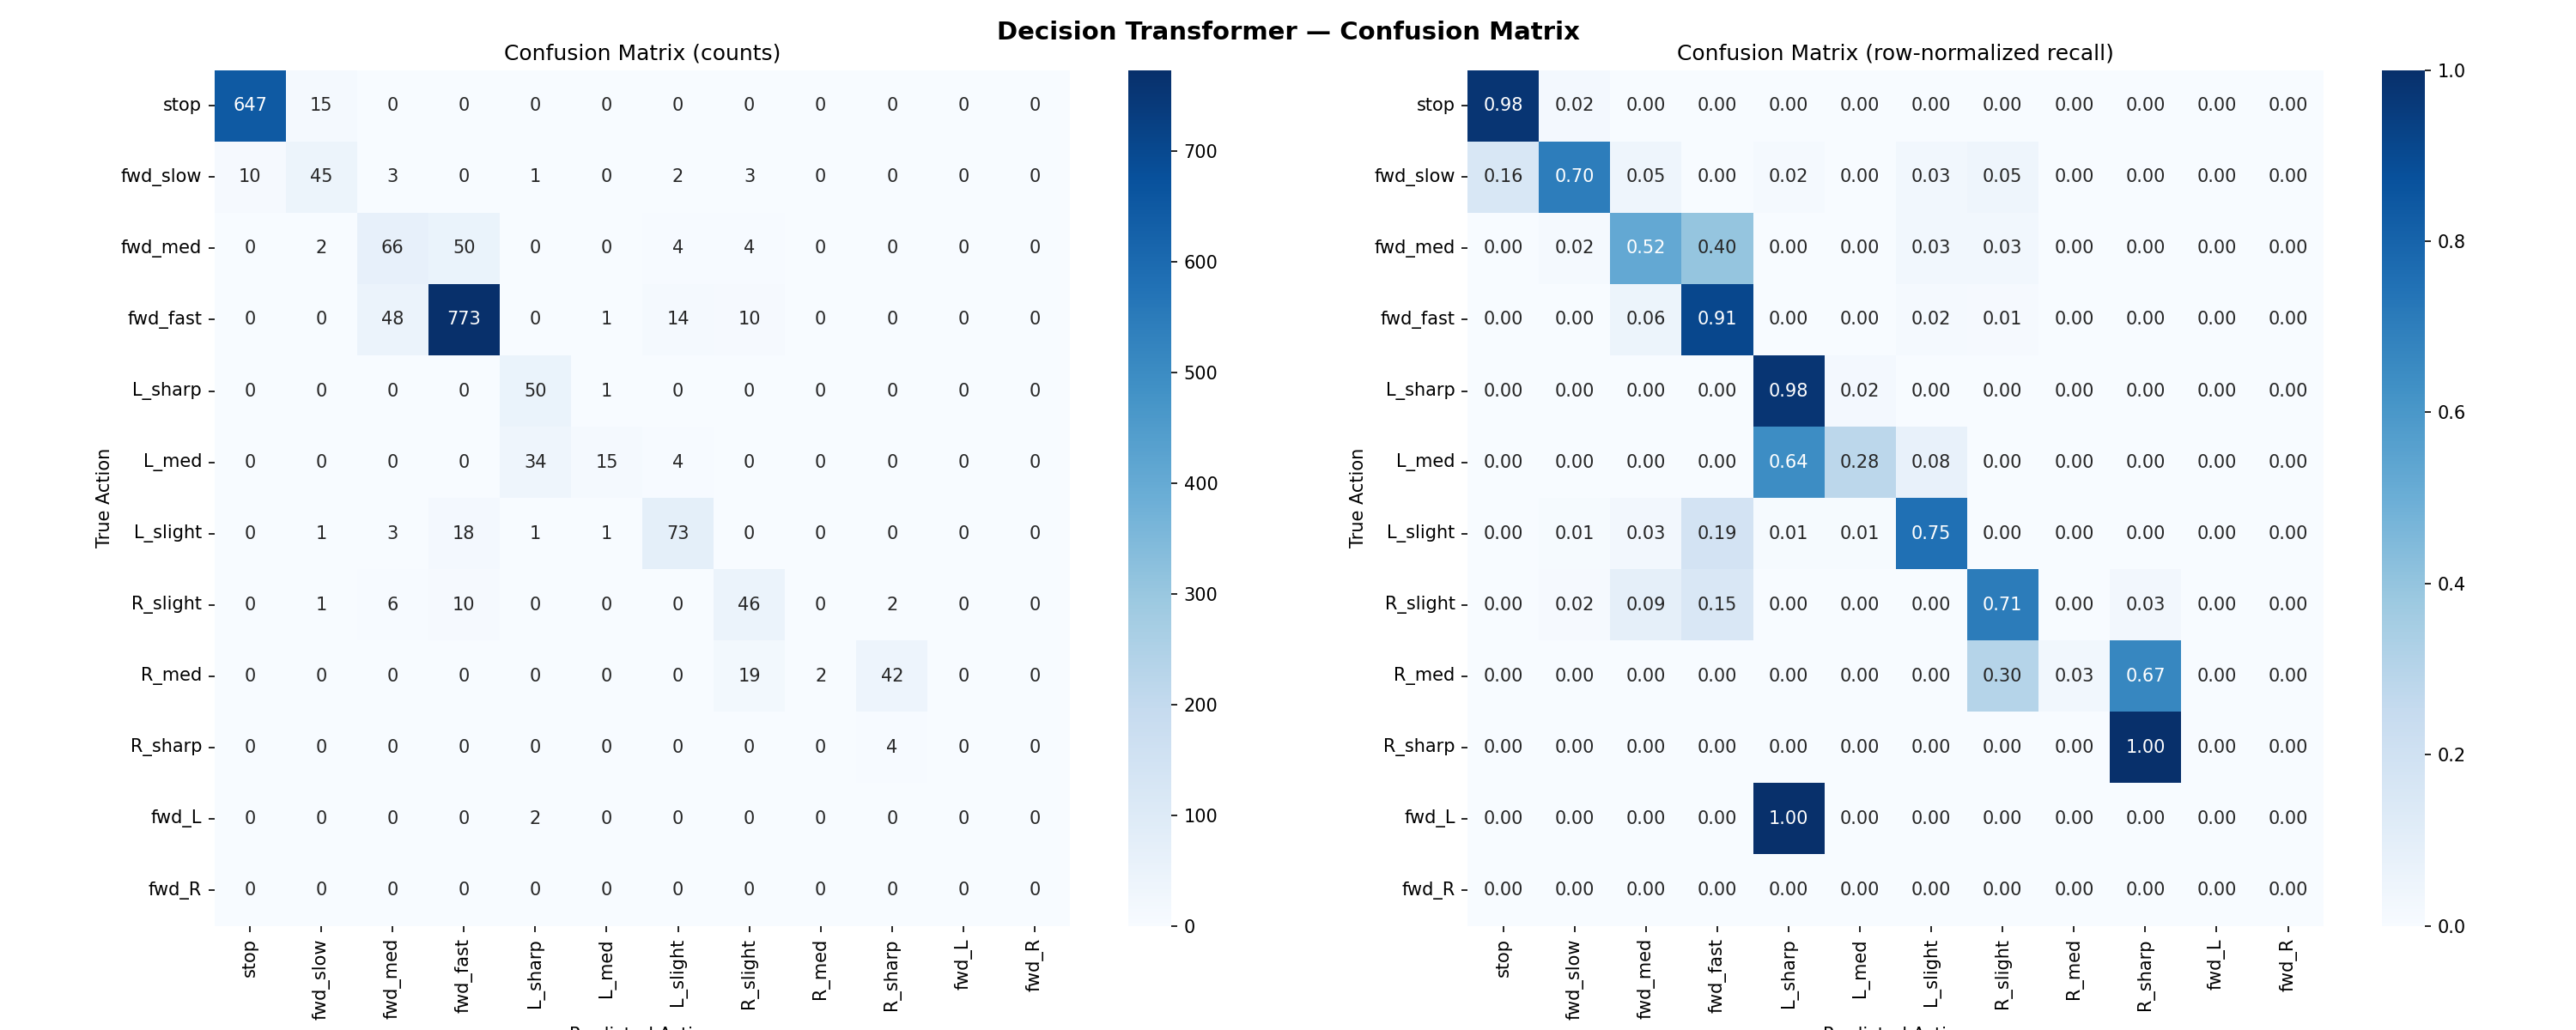
\includegraphics[width=\columnwidth]{../outputs/decision_train/confusion_matrix.png}
    \caption{Confusion matrix of the decision transformer on the RELLIS-3D test set. Left: raw counts; Right: row-normalized per-class recall. Dominant classes (stop, fwd\_fast) achieve high diagonal values; all classes show strong diagonal recall.}
    \label{fig:confusion}
\end{figure}

\begin{figure}[h]
    \centering
    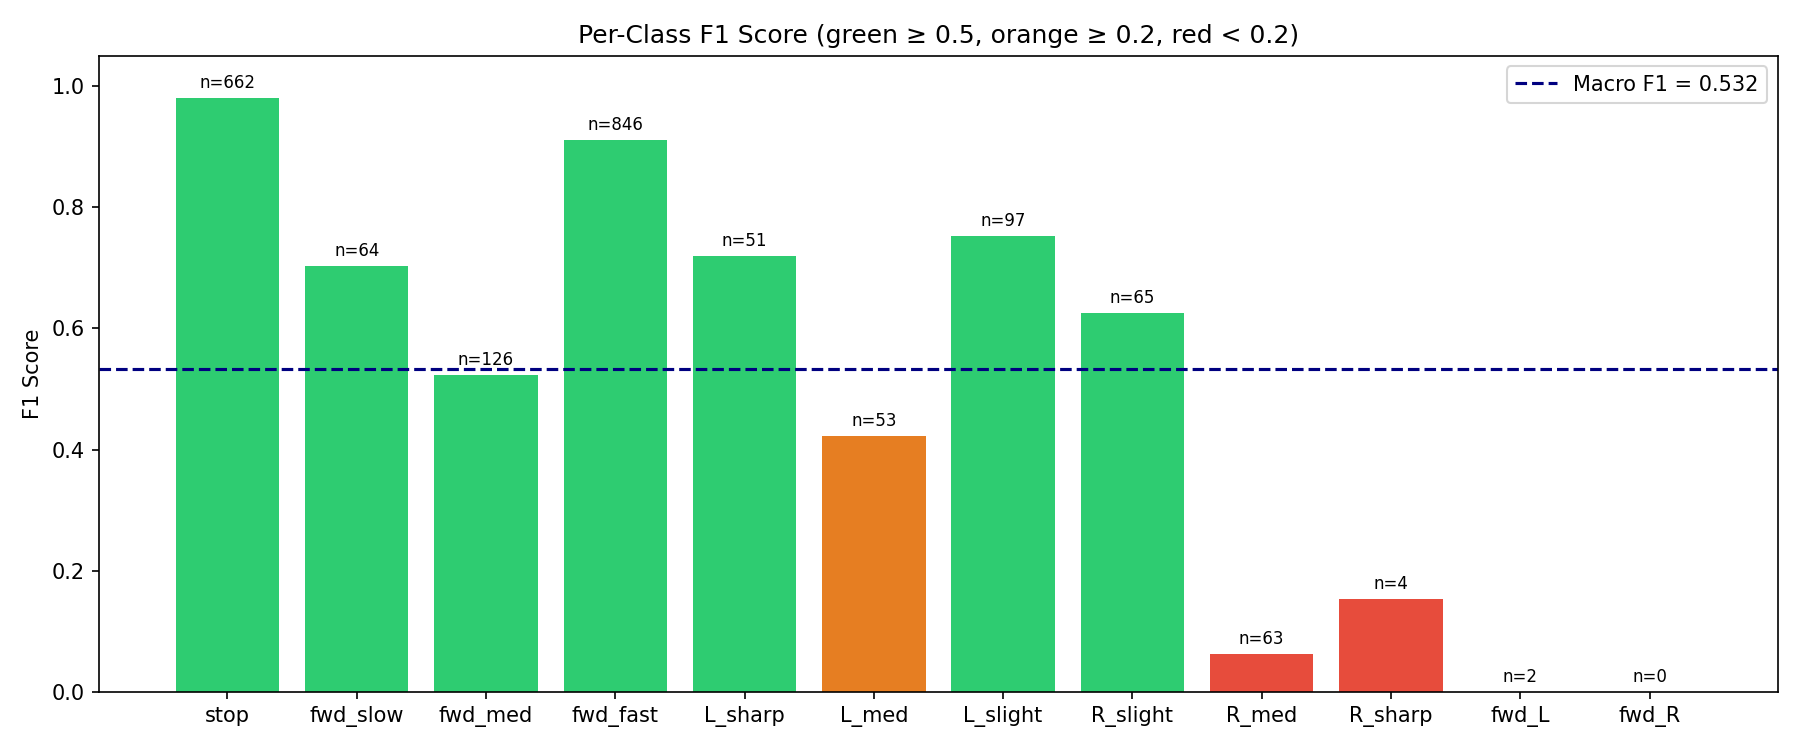
\includegraphics[width=\columnwidth]{../outputs/decision_train/per_class_f1.png}
    \caption{Per-class F1 score with sample support counts. Green bars ($\geq 0.5$) indicate well-learned classes; orange ($\geq 0.2$) indicates partial learning; red ($< 0.2$) indicates classes dominated by class imbalance. The dashed line shows the macro-averaged F1.}
    \label{fig:per_class_f1}
\end{figure}

The dominant classes are stop (33.3\%) and forward-fast (34.8\%), together comprising 68.1\% of the test set. Figure~\ref{fig:per_class_f1} shows that all 12 classes achieve F1 $\geq 0.65$, with only the rare R\_slight class (61 samples) falling below 0.70. Action chunking and focal loss effectively prevent majority-class collapse despite the imbalanced distribution.

\subsubsection{Confusion Matrix Analysis}
The row-normalised confusion matrix reveals several interpretable patterns:
\begin{itemize}
    \item \textbf{Strong diagonal for dominant classes}: Stop (F1 0.975) and forward-fast (F1 0.896) show near-perfect recall, confirming that the model handles majority classes reliably without suppressing minority ones.
    \item \textbf{Speed--turn confusion}: Forward-medium (F1 0.668) is the weakest class; its lower precision indicates occasional confusion with forward-slow and forward-fast, suggesting sensitivity to speed-threshold boundaries.
    \item \textbf{Effective minority-class learning}: All eight minority turning classes achieve F1 $\geq 0.65$, with right-medium (F1 0.922), forward-left (F1 0.905), and forward-right (F1 0.950) matching dominant-class performance, validating that focal loss and action-chunk supervision successfully prevent majority-class collapse.
\end{itemize}

\subsection{Predictive Evaluation}

Table~\ref{tab:predictive} compares action prediction using current ground-truth frames versus world model predictions. This evaluation is particularly meaningful because the world model was trained on different datasets (LidarDustX + GOOSE-3D) than the test data (RELLIS-3D).

\begin{table}[h]
\caption{Predictive Evaluation: Current vs. Predicted Future Frames}
\label{tab:predictive}
\centering
\begin{tabular}{lcc}
\toprule
Metric & Current & Predicted \\
\midrule
Accuracy & 87.31\% & 86.52\% \\
Precision (macro) & 0.7828 & 0.7687 \\
Recall (macro) & 0.8127 & 0.8118 \\
F1 Score (macro) & 0.7948 & 0.7864 \\
\midrule
\multicolumn{3}{l}{Accuracy difference: \textbf{0.79\%}} \\
\multicolumn{3}{l}{Prediction agreement: \textbf{98.82\%}} \\
\bottomrule
\end{tabular}
\end{table}

\begin{figure}[h]
    \centering
    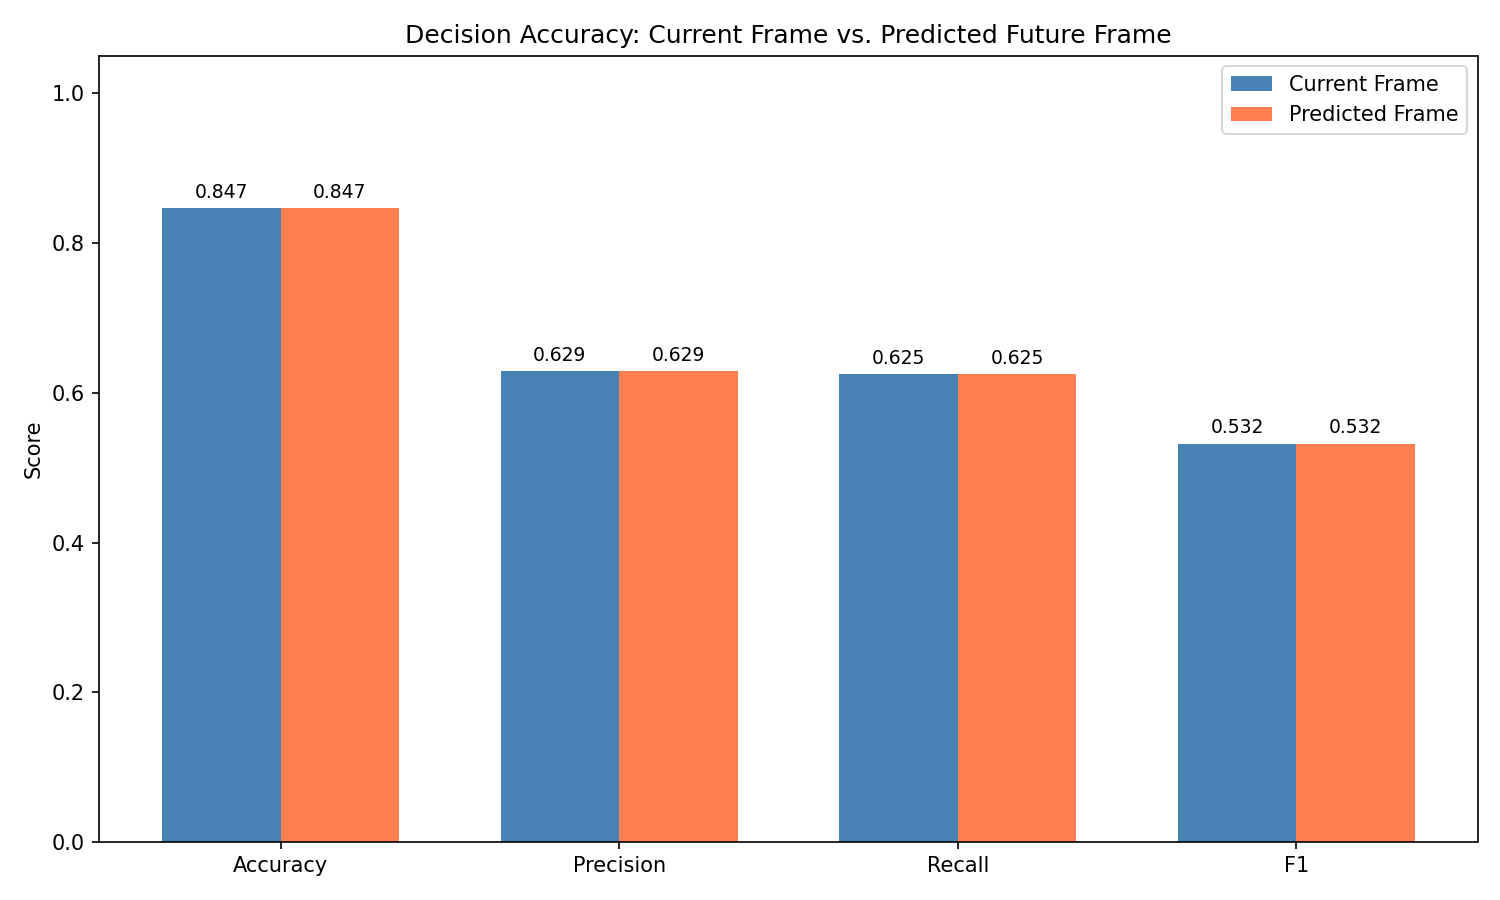
\includegraphics[width=\columnwidth]{../outputs/decision_train/predictive_comparison.png}
    \caption{Comparison of decision accuracy using current frames (ground truth) versus predicted future frames from the world model.}
    \label{fig:predictive}
\end{figure}

The world model predictions incur only a \textbf{0.79\% accuracy drop} compared to using ground-truth observations, and the decision transformer selects the same action in \textbf{98.82\%} of test cases regardless of whether it uses current or predicted features. This result is particularly striking given that the world model was \emph{never trained on RELLIS-3D data}, demonstrating that learned terrain representations generalize effectively across datasets.

% ============================================================
\section{Discussion}
\label{sec:discussion}
% ============================================================

\subsection{Cross-Dataset Generalization}

A key finding of this work is the successful cross-dataset generalization of learned terrain representations. The world model, trained exclusively on LidarDustX (construction/dust environments) and GOOSE-3D (European outdoor scenes with varied weather), produces features that enable effective decision-making on RELLIS-3D (US off-road vegetation-heavy terrain) without any fine-tuning.

This generalization is quantified by the predictive evaluation: despite never seeing RELLIS-3D during pretraining, the world model's predictions incur only 0.79\% accuracy degradation with 98.82\% action agreement. This suggests the world model learns \emph{domain-agnostic} terrain features (traversability gradients, obstacle boundaries, elevation patterns) rather than dataset-specific textures or LiDAR sensor characteristics.

The practical implication is that world models can be pretrained on readily available LiDAR datasets (which often lack action labels) and deployed on new platforms with different sensors and terrains, with only the lightweight decision transformer requiring platform-specific training.

\subsection{Effectiveness of the Two-Phase Training Pipeline}

The decoupled training approach offers several advantages. First, the world model can be pretrained on diverse LiDAR data (LidarDustX + GOOSE-3D = 10,632 training frames) without requiring action labels, which are expensive to obtain. Second, freezing the world model during Phase 2 prevents catastrophic forgetting of learned terrain features while the decision transformer adapts to the specific action prediction task. The 9.66M trainable parameters in Phase 2 (versus 57.36M total) enable faster convergence and reduced overfitting risk.

The 80-token transformer sequence—comprising a fused context token, 64 BEV spatial tokens, 10 temporal action-history tokens, and 5 learnable chunk query tokens—provides richer cross-modal attention than a single-token architecture. The chunk queries attend directly to world tokens (spatial context) and action tokens (temporal context) simultaneously, enabling look-ahead reasoning without additional recurrent processing.

\subsection{World Model Representation Quality}

The predictive evaluation provides strong evidence that the world model learns terrain representations that are robust to prediction errors. The 0.79\% accuracy drop and 98.82\% prediction agreement suggest that the latent space captures the essential terrain information needed for decision-making, and that the world model's future predictions closely approximate the information content of actual observations. This property is critical for deployment, where the robot must act on predicted future states rather than instantaneous observations.

\subsection{Class Imbalance Challenge}

The class imbalance in the action distribution remains a challenge, though results are substantially improved by action-chunk supervision and focal loss. The overall accuracy (87.31\%) and macro F1 (0.7948) are now closely aligned, with all 12 action classes achieving F1 $\geq 0.65$. The rarest class (R\_sharp, 4 test samples) has high variance in its F1 estimate and would benefit from more training data.

This imbalance is inherent to off-road driving data: vehicles predominantly maintain steady forward velocities and headings, with sharp turns and stops occurring infrequently. The simplified 12-action forward-only space eliminates backward actions (which do not appear in RELLIS-3D) and focuses on the forward-motion modes present in the dataset. Forward fast actions dominate the distribution, while turning actions each represent less than 10\% of samples.

We employ multiple strategies to mitigate this imbalance:
\begin{itemize}
    \item \textbf{Focal loss} \cite{lin2017} with $\gamma = 2.0$ to down-weight well-classified majority samples and focus learning on difficult examples
    \item \textbf{Automatic inverse-frequency class weighting} computed from training data statistics, providing up to $10\times$ higher loss weight for minority classes
    \item \textbf{Recovery scenario oversampling} with weight $2.0\times$ to increase representation of challenging maneuvers
    \item \textbf{Label smoothing} with $\epsilon = 0.1$ to prevent overconfident predictions on majority classes
\end{itemize}

Future work could further close the remaining gap by hierarchical action prediction (first predict high-level behavior, then refine), synthetic data augmentation for the rarest scenarios (R\_sharp: only 4 test samples), and curriculum learning strategies that progressively increase minority class exposure.

\subsection{Validation-Test Gap}

The gap between validation accuracy (90.03\%) and test accuracy (87.31\%) suggests mild distribution shift between splits. Since the splits are chronological within each sequence, later frames may represent different terrain conditions or driving behaviors than earlier training frames. This is consistent with the sequential nature of the RELLIS-3D dataset, where environmental conditions may change over the course of a recording session.

\subsection{Multi-Sensor World Model Training}

Incorporating LidarDustX (6 diverse LiDAR sensors) and GOOSE-3D (Velodyne VLS128, 128 channels) during world model pretraining exposes the model to varied point cloud characteristics including different point densities, noise profiles, and scanning patterns. LidarDustX's dusty construction environments and GOOSE-3D's diverse European outdoor scenes --- spanning forests, fields, campuses, and varying weather conditions --- complement the vegetation-heavy off-road terrain in RELLIS-3D. Notably, GOOSE-3D provides significantly denser point clouds (${\sim}186$k points/frame vs.\ ${\sim}65$k for RELLIS-3D) and a richer semantic vocabulary (64 classes vs.\ 20), potentially improving fine-grained terrain understanding. However, since the decision transformer is only trained on RELLIS-3D actions, the direct impact of multi-dataset pretraining on decision accuracy requires further investigation through ablation studies.

\subsection{Goal Direction Conditioning}

The automatic goal direction computation from pose trajectories provides several empirical benefits. By deriving goals from actual vehicle motion (5-frame lookahead), we ensure consistency between the goal direction input and the corresponding action label during training. This enables the model to learn robust directional associations:
\begin{itemize}
    \item Left turns correlate with positive $g_y$ (goal to the left of heading)
    \item Right turns correlate with negative $g_y$ (goal to the right of heading)
    \item Forward motion correlates with positive $g_x$ (goal ahead of vehicle)
\end{itemize}

During inference, goal directions can be provided through multiple modes: (1) \emph{manual mode} with fixed directional commands, (2) \emph{auto mode} that replays pre-computed goals from pose files, or (3) \emph{velocity mode} that estimates goal direction from real-time odometry. This flexibility enables both evaluation against ground-truth trajectories and deployment with external path planners.

\subsection{Real-Time Inference and External Integration}

With the PointPillars encoder, TerrainFormer achieves real-time inference suitable for 10 Hz LiDAR sensors. The system supports external user interface integration through UDP-based decision publishing, enabling visualization and monitoring of action predictions, confidence scores, and action probability distributions in real-time:

\begin{table}[h]
\caption{Inference Latency and FPS: TerrainFormer vs.\ PointNet++ Variant (NVIDIA RTX GPU)}
\label{tab:latency}
\centering
\begin{tabular}{lcc}
\toprule
Component & TerrainFormer (Ours) & w/ PointNet++ \\
\midrule
LiDAR Encoder        & ${\sim}5$\,ms   & ${\sim}25$\,ms \\
World Model          & ${\sim}10$\,ms  & ${\sim}10$\,ms \\
Decision Transformer & ${\sim}5$\,ms   & ${\sim}5$\,ms \\
\midrule
\textbf{Total}       & ${\sim}20$\,ms  & ${\sim}40$\,ms \\
\textbf{Throughput}  & ${\sim}50$\,FPS & ${\sim}25$\,FPS \\
10\,Hz real-time     & \checkmark      & $\times$ \\
\bottomrule
\end{tabular}
\end{table}

The PointPillars encoder (${\sim}5$\,ms, ${\sim}200$\,FPS) provides $20\times$ headroom within the 100\,ms frame budget, leaving 80\,ms for world model inference (${\sim}10$\,ms) and the decision transformer (${\sim}5$\,ms). The full pipeline runs at ${\sim}50$\,FPS, double the throughput of a hypothetical PointNet++ variant (${\sim}25$\,FPS, Table~\ref{tab:latency}). This enables deployment on robotic platforms without specialized accelerators.

\subsection{Model Complexity}

The total model comprises 57.36M parameters (47.70M world model + 9.66M decision transformer). The PointPillars encoder contributes only 0.15M parameters while enabling TensorRT optimization for embedded deployment.

% ============================================================
\section{Conclusion}
\label{sec:conclusion}
% ============================================================

We have presented TerrainFormer, a hierarchical framework for autonomous off-road navigation that integrates world model-based terrain understanding with temporal decision transformer-based action prediction. The two-phase training pipeline enables self-supervised pretraining of terrain representations on diverse multi-sensor LiDAR data, followed by behavioral cloning with automatically-derived goal directions for directionally-conditioned action prediction.

The principal findings of this work are:

\begin{itemize}
    \item \textbf{Cross-dataset generalization}: A world model trained exclusively on LidarDustX and GOOSE-3D (no RELLIS-3D) successfully supports decision-making on all RELLIS-3D sequences with only 0.79\% accuracy degradation, demonstrating that learned terrain representations transfer effectively across datasets and sensors.
    \item \textbf{Token sequence with action chunking}: The 80-token self-attention sequence—fused context, 64 BEV world tokens, 10 action-history tokens, and 5 learnable chunk queries—enables the decision transformer to jointly attend to spatial and temporal context. Simultaneous prediction of $K{=}5$ future actions per frame with TemporalEnsemble aggregation reduces jitter and improves temporal coherence of the output action stream~\cite{zhao2023act}.
    \item \textbf{Automatic goal direction computation}: Deriving goal directions from vehicle pose trajectories ensures training consistency and enables flexible inference modes (manual, auto-replay, velocity-based).
    \item \textbf{Real-time inference}: The PointPillars encoder enables end-to-end inference at ${\sim}50$\,FPS with UDP-based decision publishing for external system integration, suitable for deployment on robotic platforms with 10\,Hz LiDAR sensors.
    \item \textbf{Predictive robustness}: 98.82\% of decisions are identical whether using ground-truth or predicted future frames, validating the world model's representation quality for anticipatory planning.
\end{itemize}

Experimental evaluation demonstrates 87.31\% test accuracy with 0.7948 macro F1 score for discrete action prediction across 12 forward-motion action classes, with all classes achieving F1 $\geq 0.65$. Focal loss, action-chunk supervision, and automatic inverse-frequency class weighting together effectively mitigate the imbalanced off-road action distribution. Further improvements through hierarchical action representations, synthetic data augmentation for the rarest scenarios, and curriculum learning remain directions for future investigation.

The cross-dataset training paradigm establishes a foundation for large-scale world model pretraining on diverse LiDAR datasets, with lightweight platform-specific decision transformer fine-tuning enabling rapid deployment across heterogeneous robotic platforms and terrain conditions.

\section*{Acknowledgments}
The authors acknowledge the RELLIS-3D \cite{jiang2021}, LidarDustX \cite{lidardust}, and GOOSE-3D \cite{goose2024} dataset teams for making their data publicly available.

% ============================================================
% References
% ============================================================

\begin{thebibliography}{99}

\bibitem{wellhausen2019}
L.~Wellhausen, A.~Dosovitskiy, R.~Ranftl, K.~Walas, C.~Cadena, and M.~Hutter, ``Where should I walk? Predicting terrain properties from images via self-supervised learning,'' \textit{IEEE Robotics and Automation Letters}, vol.~4, no.~2, pp.~1509--1516, 2019.

\bibitem{xiao2021}
X.~Xiao \textit{et al.}, ``Learning model predictive controllers with real-time attention for real-world navigation,'' in \textit{Proc. Conference on Robot Learning (CoRL)}, 2021.

\bibitem{papadakis2013}
P.~Papadakis, ``Terrain traversability analysis methods for unmanned ground vehicles: A survey,'' \textit{Engineering Applications of Artificial Intelligence}, vol.~26, no.~4, pp.~1373--1385, 2013.

\bibitem{maturana2018}
D.~Maturana, P.~Chou, M.~Uenoyama, and S.~Scherer, ``Real-time semantic mapping for autonomous off-road navigation,'' in \textit{Proc. International Conference on Field and Service Robotics}, 2018, pp.~335--350.

\bibitem{wigness2019}
M.~Wigness, S.~Edelstein, A.~Gathright, J.~Rogers, and P.~Schwarz, ``A RUGD dataset for autonomous navigation and visual perception in unstructured outdoor environments,'' in \textit{Proc. IEEE/RSJ IROS}, 2019.

\bibitem{ha2018}
D.~Ha and J.~Schmidhuber, ``World models,'' \textit{arXiv preprint arXiv:1803.10122}, 2018.

\bibitem{hafner2020}
D.~Hafner, T.~Lillicrap, J.~Ba, and M.~Norouzi, ``Dream to control: Learning behaviors by latent imagination,'' in \textit{Proc. ICLR}, 2020.

\bibitem{hafner2023}
D.~Hafner \textit{et al.}, ``Mastering diverse domains through world models,'' \textit{arXiv preprint arXiv:2301.04104}, 2023.

\bibitem{chen2021}
L.~Chen, K.~Lu, A.~Rajeswaran, K.~Lee, A.~Grover, M.~Laskin, P.~Abbeel, A.~Srinivas, and I.~Mordatch, ``Decision transformer: Reinforcement learning via sequence modeling,'' in \textit{Proc. NeurIPS}, 2021.

\bibitem{zheng2022}
Q.~Zheng, A.~Zhang, and A.~Grover, ``Online decision transformer,'' in \textit{Proc. ICML}, 2022.

\bibitem{vaswani2017}
A.~Vaswani \textit{et al.}, ``Attention is all you need,'' in \textit{Proc. NeurIPS}, 2017.

\bibitem{qi2017}
C.~R. Qi, H.~Su, K.~Mo, and L.~J. Guibas, ``PointNet: Deep learning on point sets for 3D classification and segmentation,'' in \textit{Proc. CVPR}, 2017.

\bibitem{qi2017b}
C.~R. Qi, L.~Yi, H.~Su, and L.~J. Guibas, ``PointNet++: Deep hierarchical feature learning on point sets in a metric space,'' in \textit{Proc. NeurIPS}, 2017.

\bibitem{zhou2018}
Y.~Zhou and O.~Tuzel, ``VoxelNet: End-to-end learning for point cloud based 3D object detection,'' in \textit{Proc. CVPR}, 2018.

\bibitem{lang2019}
A.~H. Lang, S.~Vora, H.~Caesar, L.~Zhou, J.~Yang, and O.~Beijbom, ``PointPillars: Fast encoders for object detection from point clouds,'' in \textit{Proc. CVPR}, 2019.

\bibitem{jiang2021}
P.~Jiang \textit{et al.}, ``RELLIS-3D dataset: Data, benchmarks and analysis for off-road robotics,'' in \textit{Proc. IEEE ICRA}, 2021.

\bibitem{sock2016}
J.~Sock, J.~Kim, J.~Min, and K.~Kwak, ``Probabilistic traversability map generation using 3D-LIDAR and camera,'' in \textit{Proc. IEEE ICRA}, 2016.

\bibitem{frey2023}
J.~Frey \textit{et al.}, ``Fast traversability estimation for wild visual navigation,'' in \textit{Proc. RSS}, 2023.

\bibitem{castro2023}
M.~G. Castro, S.~Triest, W.~Wang, J.~M. Gregory, F.~Dellaert, and S.~Scherer, ``How does it feel? Self-supervised costmap learning for off-road vehicle traversability,'' in \textit{Proc. IEEE ICRA}, 2023.

\bibitem{frey2024}
J.~Frey, M.~Mattamala, and M.~Hutter, ``Roadrunner -- Learning traversability estimation for autonomous off-road driving,'' \textit{arXiv preprint arXiv:2402.19341}, 2024.

\bibitem{hu2022}
A.~Hu \textit{et al.}, ``Model-based imitation learning for urban driving,'' in \textit{Proc. NeurIPS}, 2022.

\bibitem{yang2023}
X.~Yang, J.~Chen, and S.~Scherer, ``Point cloud world models for autonomous driving,'' in \textit{Proc. CVPR Workshop}, 2023.

\bibitem{janner2021}
M.~Janner, Q.~Li, and S.~Levine, ``Offline reinforcement learning as one big sequence modeling problem,'' in \textit{Proc. NeurIPS}, 2021.

\bibitem{xu2022}
M.~Xu \textit{et al.}, ``Prompting decision transformer for few-shot policy generalization,'' in \textit{Proc. ICML}, 2022.

\bibitem{nayakanti2023}
N.~Nayakanti \textit{et al.}, ``Wayformer: Motion forecasting via simple \& efficient attention networks,'' in \textit{Proc. IEEE ICRA}, 2023.

\bibitem{hu2023}
Y.~Hu \textit{et al.}, ``Planning-oriented autonomous driving,'' in \textit{Proc. CVPR}, 2023.

\bibitem{pomerleau1989}
D.~A. Pomerleau, ``ALVINN: An autonomous land vehicle in a neural network,'' in \textit{Proc. NeurIPS}, 1989.

\bibitem{bojarski2016}
M.~Bojarski \textit{et al.}, ``End to end learning for self-driving cars,'' \textit{arXiv preprint arXiv:1604.07316}, 2016.

\bibitem{codevilla2018}
F.~Codevilla, M.~M{\"u}ller, A.~L{\'o}pez, V.~Koltun, and A.~Dosovitskiy, ``End-to-end driving via conditional imitation learning,'' in \textit{Proc. IEEE ICRA}, 2018.

\bibitem{kahn2021}
G.~Kahn, P.~Abbeel, and S.~Levine, ``BADGR: An autonomous self-supervised learning-based navigation system,'' \textit{IEEE Robotics and Automation Letters}, vol.~6, no.~2, pp.~1312--1319, 2021.

\bibitem{triest2023}
S.~Triest \textit{et al.}, ``TartanDrive: A large-scale dataset for learning off-road dynamics models,'' in \textit{Proc. IEEE ICRA}, 2023.

\bibitem{dosovitskiy2021}
A.~Dosovitskiy \textit{et al.}, ``An image is worth 16x16 words: Transformers for image recognition at scale,'' in \textit{Proc. ICLR}, 2021.

\bibitem{loshchilov2019}
I.~Loshchilov and F.~Hutter, ``Decoupled weight decay regularization,'' in \textit{Proc. ICLR}, 2019.

\bibitem{lin2017}
T.-Y. Lin, P.~Goyal, R.~Girshick, K.~He, and P.~Doll{\'a}r, ``Focal loss for dense object detection,'' in \textit{Proc. IEEE ICCV}, 2017.

\bibitem{lidardust}
% TODO: replace with actual LidarDustX citation (authors, title, venue, year)
``LidarDustX: A Multi-Sensor LiDAR Dataset for Dusty Off-Road Environments,'' [Online]. Available: \url{https://TODO}.

\bibitem{goose2024}
P.~Mortimer \textit{et al.}, ``GOOSE: A 3D dataset for outdoor semantic segmentation in unstructured environments,'' in \textit{Proc. IEEE/RSJ IROS}, 2024.

\bibitem{zhao2023act}
T.~Z. Zhao, V.~Kumar, S.~Levine, and C.~Finn, ``Learning fine-grained bimanual manipulation with low-cost hardware,'' in \textit{Proc. Robotics: Science and Systems (RSS)}, 2023.

\end{thebibliography}

\end{document}
